\documentclass[
   %handout
 ]{beamer}
 
\usetheme{simple}
\usepackage{lmodern}
\usepackage[scale=2]{ccicons}

%Codifica dei font di input e di output
\usepackage[T1]{fontenc}
\usepackage[utf8]{inputenc}

% Converte file eps in pdf
\usepackage{epstopdf}

% Consente di impostare le virgolette del discorso diretto
\usepackage{dirtytalk}

% Consente di impostare i commenti multiline
\usepackage{verbatim}

% Consente di disegnare grafi
\usepackage{tikz}

% Libreria per disegnare cerchi e frecce di tikz
\usetikzlibrary{arrows}

% Definizione della cartella contenente le immagini da usare
\graphicspath{{img/}}

% Disabilitare la trasparenza sulla pause
\setbeamercovered{invisible}
            
% TODO
% Finire Parte algoritmo di apprendimento
% Backpropagation
% Migliorare la spiegazione delle slide


% Watermark background (simple theme)
%\setwatermark{\includegraphics[height=8cm]{img/Heckert_GNU_white.png}}
     
%\institute{\url{http://github.com/famuvie}}

% Metadati di apertura del pdf
\hypersetup{
    pdftoolbar=true,        % show Acrobat’s toolbar?
    pdfmenubar=true,        % show Acrobat’s menu?
    pdffitwindow=false,     % window fit to page when opened
    pdfstartview={FitH},    % fits the width of the page to the window
    pdfencoding=auto
}

% Definizione degli autori
\author {
            \texorpdfstring{\hspace*{0.01em}{\Large Michele Valsesia}}{Michele Valsesia} 
            \texorpdfstring{\\ \bigskip}{e}
            \texorpdfstring{\hspace*{0.3em}{\Large Nicholas Aspes }}{Nicholas Aspes}
        }

\begin{document}

% Definizione del Titolo e Anno Accademico

\title{Implementazione di una \\ 
       Rete Convoluzionale in CUDA \bigskip}
        
\date{\Large Anno accademico 2018/2019}


% Titolo della Presentazione
     
\begin{frame}
\maketitle
\end{frame}

% //////////////////////////////// Introduzione ////////////////////////////////////////


\begin{frame}{Introduzione}
    \framesubtitle{Obiettivi}  
    
    \begin{itemize} [<+->]
        \setlength\itemsep{2em}
        \item \large Descrivere brevemente l'architettura ed il funzionamento di una \emph{Rete Neurale}
        \item \large Motivare le differenti scelte implementative adottate durante lo svolgimento del progetto
        \item \large Valutare l'accuratezza e lo speed-up della rete rispetto ad una sua implementazione sequenziale       
    \end{itemize}  
\end{frame}


% //////////////////////////////// Parte Teorica Reti Neurali //////////////////////////

\begin{frame}[c]
  \centering
  \bigskip \bigskip    
  \Huge Reti Neurali
\end{frame}

\begin{frame}{Reti Neurali}
    \framesubtitle{Scopo}
    \begin{itemize} [<+->]
        \setlength\itemsep{2em}
        \item \large Le \emph{Reti Neurali} vengono principalmente usate per la classificazione delle immagini
       \item \large Il processo di classificazione consiste nell'associare ad un'immagine un'etichetta che identifica nel miglior modo possibile il suo contenuto semantico
       \item \large Una \emph{classe} non è altro che l'etichetta di un'immagine
       \item \large Le reti neurali ricevono in input un'immagine e forniscono in output la relativa classe 
    \end{itemize}
\end{frame} 

\begin{frame}{Reti Neurali}
    \framesubtitle{Apprendimento}
    \begin{itemize} [<+->]
        \setlength\itemsep{2em}
        \item \large Per poter classificare, una rete neurale deve \emph{imparare} ad associare correttamente le immagini alle varie classi
        \item \large Il \emph{training set} ed il \emph{test set} sono due insiemi composti da coppie (immagini, etichette) chiamate \emph{esempi}
        \item \large Le etichette di ciascun esempio vengono assegnate in maniera soggettiva da personale umano 
    \end{itemize}
\end{frame}

\begin{frame}{Reti Neurali}
    \framesubtitle{Training Set}
    \begin{itemize} [<+->]
        \setlength\itemsep{2em}
        \item \large Il training set viene usato durante la fase di apprendimento della rete
        \item \large Per ognuno degli esempi del training set
        
        \smallskip
        
        \setbeamertemplate{itemize items}[square] 
        \begin{itemize} 
        \setlength\itemsep{1em}
            \item \large La rete riceve in input l'immagine dell'esempio considerato e l'associa ad una delle classi presenti
            \item \large Se la classe di output non corrisponde all'etichetta dell'esempio, la rete corregge i suoi parametri interni e passa all'immagine successiva
        \end{itemize}
    \end{itemize}
\end{frame}

\begin{frame}{Reti Neurali}
    \framesubtitle{Test Set}
    \begin{itemize} [<+->]
        \setlength\itemsep{2em}
        \item \large Il test set verifica che la rete abbia imparato a discriminare correttamente le immagini
        \item \large Viene valutata l'\emph{accuratezza} della rete come il rapporto tra il numero di esempi classificati scorrettamente ed il numero totale di esempi
        
        \item \large Per ognuno degli esempi del test set
        
        \smallskip
        
        \setbeamertemplate{itemize items}[square] 
        \begin{itemize} 
        \setlength\itemsep{1em}
            \item \large La rete riceve in input l'immagine dell'esempio considerato e l'associa ad una delle classi presenti
            \item \large Ogni volta che l'output della rete non corrisponde all'etichetta dell'esempio, viene incrementato un contatore, necessario al calcolo dell'accuratezza
        \end{itemize}
    \end{itemize}
\end{frame}

\begin{frame}{Reti Neurali}
    \framesubtitle{Significato Biologico}
    \begin{itemize} [<+->]
        \setlength\itemsep{2em}
        \item \large Le \emph{Reti Neurali} nascono con lo scopo di modellare una rete neurale biologica
       \item \large Una rete neurale biologica si compone di unità cellulari di base: i \emph{neuroni}
       \item \large I neuroni sono collegati tra loro per mezzo di specifiche giunture chiamate \emph{sinapsi}
    \end{itemize}
\end{frame} 

\begin{frame}{Reti Neurali}
    \framesubtitle{Neurone}
    
    \begin{center}
      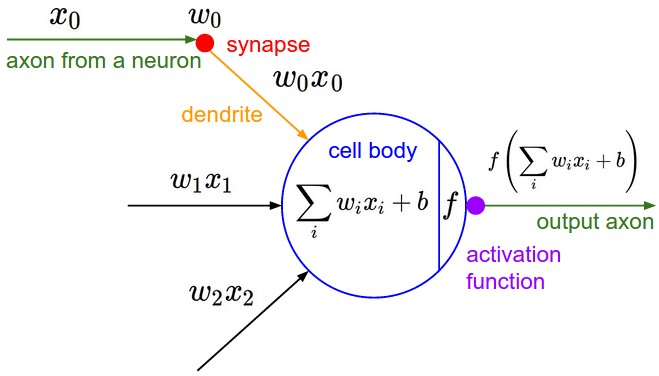
\includegraphics[scale = 0.35]{neuron_model.jpeg}
    \end{center}
  
    \bigskip 
  
  \begin{itemize}
    \setlength\itemsep{1em}
    \item[] \large \emph{Modello matematico di un neurone}
  \end{itemize}       
\end{frame} 


\begin{frame}{Reti Neurali}
    \framesubtitle{Funzionamento Neurone}
    \begin{itemize} [<+->]
        \setlength\itemsep{2em}
        \item \large Attraverso un meccanismo di eccitazione ed inibizione i pesi sinaptici controllano quanto un neurone venga influenzato dagli altri
       \item \large I segnali pesati dalle differenti sinapsi vengono trasportati dai dendriti all'interno del neurone e sommati tra loro
       \item \large Se la somma supera una certa soglia, il neurone \emph{spara} un segnale lungo l'assone 
       \item \large La \emph{frequenza di sparo} del neurone viene modellata con una funzione di attivazione $f$       
    \end{itemize}
\end{frame}


\begin{frame}{Reti Neurali}
    \framesubtitle{Funzioni di Attivazione}
    \begin{block}{Definizione} 
        \large Una \emph{funzione di attivazione} è una funzione matematica non lineare usata per calcolare l'output di un neurone. Riceve come input la somma pesata dei segnali in ingresso al neurone
    \end{block}\pause
    
    \begin{itemize} [<+->]
        \setlength\itemsep{2em}
        \item \emph{\large Sigmoide}
        \item \emph{\large Tangente Iperbolica}
        \item \emph{\large Softplus}
    \end{itemize}
\end{frame}

\begin{frame}{Reti Neurali}
    \framesubtitle{Sigmoide}
    \begin{block}{Definizione} 
        \large La \emph{Sigmoide} $\sigma: \mathbb{R} \rightarrow [0, 1]$ è definita come $\sigma(x) = \frac{1}{(1 + e^{-x})}$ 
    \end{block}\pause
    
    \begin{itemize} [<+->]
        \setlength\itemsep{2em}
        \item \large Per elevati valori negativi di input la sigmoide restituisce 0: il neurone non spara affatto
        \item \large Per elevati valori positivi di input la sigmoide restituisce 1: il neurone satura e spara con una frequenza di sparo pari a 1
        \item \large La sua derivata è uguale a $\sigma^{\prime}(x) = 1 - \sigma(x)$
    \end{itemize}
\end{frame}

\begin{frame}{Reti Neurali}
    \framesubtitle{Sigmoide}
    
    \begin{center}
      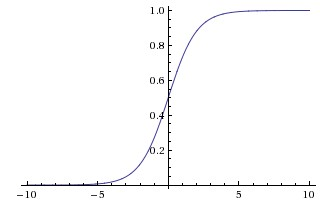
\includegraphics[scale = 0.6]{sigmoid.jpeg}
    \end{center}
  
    \bigskip 
  
  \begin{itemize}
    \setlength\itemsep{1em}
    \item[] \large \emph{Rappresentazione grafica Sigmoide}
  \end{itemize}       
\end{frame} 



\begin{frame}{Reti Neurali}
    \framesubtitle{Tangente Iperbolica}
    \begin{block}{Definizione} 
        \large La \emph{Tangente Iperbolica} $\tanh: \mathbb{R} \rightarrow [-1, 1]$ è definita come $\tanh(x) = 2\sigma(2x) - 1$ 
    \end{block}\pause
    
    \begin{itemize} [<+->]
        \setlength\itemsep{2em}
        \item \large La tangente iperbolica è una sigmoide scalata 
        \item \large La sua derivata è uguale a $\tanh^{\prime}(x) = 1 - \tanh^{2}(x)$
    \end{itemize}
\end{frame}

\begin{frame}{Reti Neurali}
    \framesubtitle{Tangente Iperbolica}
    
    \begin{center}
      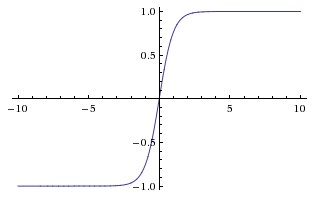
\includegraphics[scale = 0.6]{tanh.jpeg}
    \end{center}
  
    \bigskip 
  
  \begin{itemize}
    \setlength\itemsep{1em}
    \item[] \large \emph{Rappresentazione grafica Tangente Iperbolica}
  \end{itemize}       
\end{frame} 

\begin{frame}{Reti Neurali}
    \framesubtitle{Softplus}
    \begin{block}{Definizione} 
        \large La \emph{Softplus} $s: \mathbb{R} \rightarrow [0, +\infty]$ è definita come $s(x) = \log(1 + e^x)$ 
    \end{block}\pause
    
    \begin{itemize} [<+->]
        \setlength\itemsep{2em}
        \item \large La softplus è un approssimazione della \emph{Rectifier Linear Unit (ReLU)}
        \item \large Viene usata per sostituire la ReLU che presenta un punto di discontinuità in 0
        \item \large La sua derivata è uguale a $s^{\prime}(x) = \frac{1}{(1 + e^{-x})}$
    \end{itemize}
\end{frame}

\begin{frame}{Reti Neurali}
    \framesubtitle{Softplus}
    
    \begin{center}
      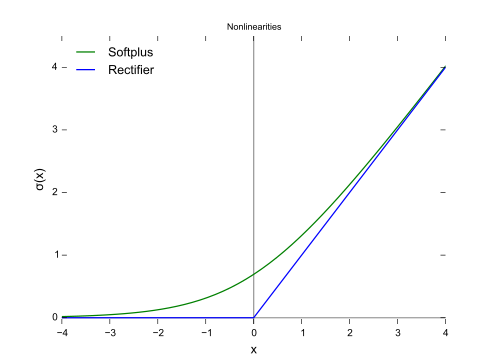
\includegraphics[scale = 0.45]{softplus_vs_rectifier.png}
    \end{center}
  
    \smallskip
  
  \begin{itemize}
    \setlength\itemsep{1em}
    \item[] \large \emph{Confronto grafico tra ReLU e Softplus}
  \end{itemize}       
\end{frame} 

\begin{frame}{Reti Neurali}
    \framesubtitle{Rete Neurale}
    
    \begin{block}{Definizione} 
        \large Una \emph{Rete Neurale} è composta da un insieme di neuroni connessi tra loro in un grafo aciclico
    \end{block}\pause
    
    \begin{itemize} [<+->]
        \setlength\itemsep{2em}
        \item \large  I neuroni sono organizzati in insiemi distinti chiamati \emph{livelli} o \emph{layer}
        \item \large I livelli vengono posti uno di seguito all'altro in modo da formare una sequenza
        \item \large I livelli intermedi prendono il nome di \emph{hidden}
        \item \large L'output dei neuroni di un livello diventano l'input dei neuroni del livello successivo        
    \end{itemize}
\end{frame}

\begin{frame}{Reti Neurali}
    \framesubtitle{Rete Neurale}
    
    \begin{itemize} [<+->]
        \setlength\itemsep{2em}
        \item \large Quando si effettua il conteggio dei livelli di una rete non si considera il livello di input
        \item \large Una rete a \emph{singolo livello} non presenta livelli hidden    
        \item \large Per determinare la grandezza di una rete ci si concentra sul numero di neuroni e sui relativi pesi ad essi associati
    \end{itemize}
\end{frame}

\begin{frame}{Reti Neurali}
    \framesubtitle{Livello Fully-Connected}
    
    \begin{block}{Definizione} 
        \large Un livello è di tipo \emph{Fully-Connected} quando i neuroni appartenenti a due livelli adiacenti sono completamente connessi tra loro mentre i neuroni associati ad un singolo livello non condividono nessuna connessione 
    \end{block}\pause
    
    \begin{itemize} [<+->]
        \setlength\itemsep{2em}
        \item \large I pesi dei neuroni di un livello vengono salvati all'interno di matrici
        \item \large Le righe della matrice identificano i neuroni del livello mentre le colonne rappresentano i pesi di ciascun neurone
        \item \large La struttura a livelli di una rete neurale consente di facilitare le varie operazioni sfruttando il calcolo matriciale 
    \end{itemize}
\end{frame}

\begin{frame}{Reti Neurali}
    \framesubtitle{Livello Fully-Connected}
    
    \begin{center}
      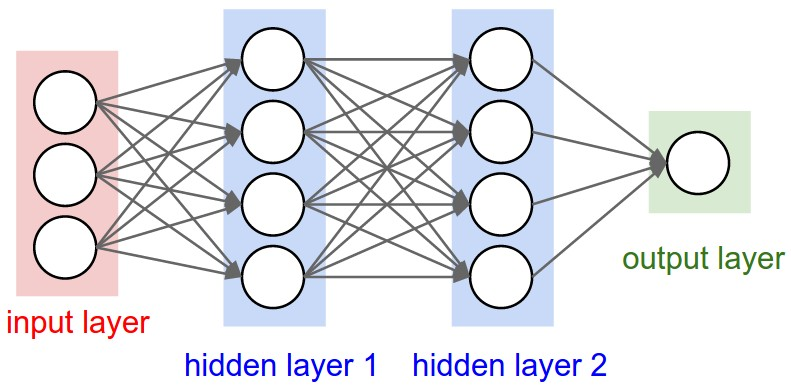
\includegraphics[scale = 0.4]{fully_connected.jpeg}
    \end{center}
  
    \smallskip
  
    \begin{itemize}
        \setlength\itemsep{1em}
        \item[] \large \emph{Una rete neurale a 3 livelli}
    \end{itemize}       
\end{frame} 



\begin{frame}{Reti Neurali}
    \framesubtitle{Funzionamento}
    
    Il processo di apprendimento di una rete neurale è suddiviso in quattro fasi distinte \pause
    
    \begin{itemize} [<+->]
        \setlength\itemsep{2em}
        \item \emph{\large Inizializzazione dei pesi}
        \item \emph{\large Forward Propagation}
        \item \emph{\large Funzione di perdita}
        \item \emph{\large Back Propagation}
    \end{itemize}
\end{frame}

\begin{frame}{Reti Neurali}
    \framesubtitle{Inizializzazione dei pesi}
    
    \begin{itemize} [<+->]
        \setlength\itemsep{2em}
        \item \large Al momento della nascita gli esseri umani non sono in grado di discriminare nessun tipo di oggetto a causa del mancato addestramento della loro rete neurale biologica
        \item \large Per riprodurre questo comportamento, all'inizio della fase di training, i pesi sinaptici $w_i$ di ciascun livello vengono inizializzati in maniera casuale     
    \end{itemize}
\end{frame}



\begin{frame}{Reti Neurali}
    \framesubtitle{Forward Propagation}
    
    \begin{block}{Definizione} 
        \large La \emph{Forward Propagation} è il meccanismo utilizzato da una rete neurale per associare un'immagine ad una determinata classe
    \end{block}\pause
        
    \begin{itemize} [<+->]
        \setlength\itemsep{2em}
        \item \large L'output dei neuroni del livello $i$ viene moltiplicato per la matrice dei pesi del livello $i+1$ ottenendo il vettore $v$
        \item \large Al vettore $v$ viene aggiunto il vettore dei bias del livello $i+1$
        \item \large L'output del livello $i+1$ si ottiene applicando la funzione di attivazione $f$ ad ogni entry del vettore $v$
        \item \large Le operazioni precedenti sono svolte per tutti i livelli ad eccezione dell'ultimo
    \end{itemize}
\end{frame}

\begin{frame}{Reti Neurali}
    \framesubtitle{Funzione di perdita}
    
    \begin{block}{Definizione} 
        \large Una \emph{funzione di perdita} $L$ serve per determinare l'errore di classificazione di una rete neurale
    \end{block}\pause
        
    \begin{itemize} [<+->]
        \setlength\itemsep{2em}
        \item \large La funzione di perdita più usata è la \emph{Mean Squared Error (MSE)} $L = \frac{1}{2} \sum (target - output)^{2}$
        \item \large Per ridurre l'errore di una rete neurale è necessario minimizzare la funzione $L$
        \item \large Il valore minimo di $L$ si ottiene calcolando la sua derivata rispetto ai pesi, il cosiddetto \emph{gradiente} 
    \end{itemize}
\end{frame}

\begin{frame}{Reti Neurali}
    \framesubtitle{Funzione di perdita}
    
    \begin{center}
      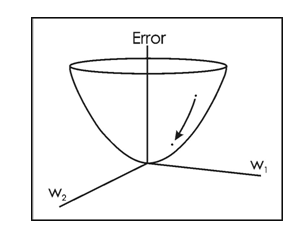
\includegraphics[scale = 0.8]{Loss.png}
    \end{center}
  
    \smallskip
  
    \begin{itemize}
        \setlength\itemsep{1em}
        \item[] \large \emph{Mean Squared Error (MSE). I pesi $w_1$ e $w_2$ sono le variabili indipendenti mentre la variabile dipendente è la funzione di perdita $L$}
    \end{itemize}       
\end{frame} 

\begin{frame}{Reti Neurali}
    \framesubtitle{Back Propagation}
    
    \begin{itemize} [<+->]
        \setlength\itemsep{2em}
        \item \large Lo scopo della back propagation consiste nel trovare, per ogni livello, i pesi $w$ che minimizzino una funzione di perdita $L$
    \end{itemize}
\end{frame}




\begin{frame}{Reti Neurali}
    \framesubtitle{Rete Neurale Convoluzionale}  
    Una \emph{Rete Neurale Convoluzionale} si differenzia da una più classica in quanto assume che l'input della rete sia un'immagine
\end{frame}   

\begin{frame}[c]
  \centering
  \bigskip \bigskip    
  \Huge Implementazione della Rete
\end{frame}

\begin{frame}[c]
  \centering
  \bigskip \bigskip    
  \Huge Analisi dei Risultati
\end{frame}


\end{document}
